\documentclass{beamer}
\usefonttheme{serif}
\usefonttheme{professionalfonts}
\usepackage[latin1]{inputenc}
\usepackage[T1]{fontenc}
\usepackage{hhline,bm,xspace,url}
\usepackage[expert,seriftt]{lucidabr}
\renewcommand{\rmdefault}{hlhj}
\usepackage{fancyvrb}
\usepackage{url,xcolor,ctable}
\usepackage{marvosym}
\usepackage{tikz}
\usepackage{listings}
\lstset{frame=lines,basicstyle=\ttfamily,showspaces=true,prebreak={\Righttorque},postbreak={\Lefttorque},breaklines}
\newcommand{\tl}{\TeX~Live}
\newcommand{\tpm}{\texttt{tpm}}
\newcommand{\tpms}{\tpm{}s}
\newcommand{\tlpsrc}{\texttt{tlpsrc}}
\newcommand{\tlpsrcs}{\tlpsrc{}s}
\newcommand{\tlpobj}{\texttt{tlpobj}}
\newcommand{\tlpobjs}{\tlpobj{}s}
\newcommand{\tlpdb}{\texttt{tlpdb}}
\newcommand{\tlpdbs}{\tlpdb{}s}
\newcommand{\tlmgr}{\tl~Manager}
\newcommand{\acro}[1]{\textsc{\MakeLowercase{#1}}}
\newcommand{\ctan}{\acro{CTAN}}
\newcommand{\cmd}[1]{\textsf{#1}}
\newcommand{\button}[1]{\textsf{#1}}
\newcommand{\var}[1]{\textsl{#1}}
\newcommand{\XeTeX}{Xe\TeX}

\def\bigit{\\[\bigskipamount]}
\def\medit{\\[\medskipamount]}

\hyphenation{infra-struc-ture}
\DefineShortVerb{\|}

\usetheme[headheight=75pt,footheight=10pt]{boxes}
\setbeamercolor*{black on white}{bg=white,fg=black}
%\setbeamerfont*{black on white}{series=\scshape}
\addfootbox{black on white}{\hbox{\vbox to 10pt{%
      %\hspace{3em}Norbert 
      % Preining, \tl~2008 -- {\normalfont Brno, CSTUG Meeting 2008}
      \hfill \insertframenumber\hspace{3em}~~\vfill}}}
\addheadbox{black on white}{
\includegraphics{texlive2008-logo-2.png}}
\setbeamertemplate{navigation symbols}{}

\setlength{\parskip}{\medskipamount}

\def\cred#1{{\color{red}#1}}
\def\cblue#1{{\usebeamercolor[fg]{structure}#1}}
\def\prog#1{\texttt{#1}}

\def\img#1#2#3#4{%
  \bgroup%
  \setbox0=\hbox{\hskip #3\vbox to 0pt{\vskip #4 \includegraphics[height=#2]{#1}}}%
  \dp0=0pt %
  \ht0=0pt %
  \wd0=0pt %
  %\hbox to \textwidth{\hfill\hbox{\box0}}%
  \hbox{\box0}
  \egroup}


%%%%%%%%%%%%%%%%%%%%%%%%%%%%%%%%%%%%%%%%%%%%%%%%%%%%%%%%%%%%%%%%%%
%
% here begins the stuff
%
%%%%%%%%%%%%%%%%%%%%%%%%%%%%%%%%%%%%%%%%%%%%%%%%%%%%%%%%%%%%%%%%%%%%
\title{} %\tl~2008}
\title{Norbert Preining}
%\author{Norbert Preining}
\author{Vienna University of Technology, Austria\\[\bigskipamount]
\textsc{cstug Meeting 2008, Brno, Czech Republic}}
\date{13 December 2008}

%Bachotek, Poland \hspace{\bigskipamount} 13~December 2008}

\begin{document}

\frame{\titlepage}

\begin{frame}
  \frametitle{Layout}
  \begin{center}
    \begin{tabular}[h!]{ll}
      \cblue{Part for users} & \cblue{Technical part} \\
      \midrule
      Overview  & Getting things into \tl \\
      Installation & The new infrastructure \\
      \tlmgr \qquad\qquad & Internals of the \tlpdb, config options\\
      Other news
    \end{tabular}
  \end{center}
\end{frame}

\section{Users' perspective}

\subsection{Overview}

\begin{frame}
  \frametitle{History}
  \begin{itemize}
  \item late 1993 Dutch \TeX\ Users Group, 4All\TeX\ CD, \acro{tds}
    working group\pause
  \item 1995 Unix-based \acro{TDS} \acro{CD} based on te\TeX\pause
  \item 1996 first edition, Sebastian Rahtz%
    \uncover<3-3>{\img{rahtz.png}{110pt}{10pt}{-5pt}}\pause
  \item 2000 5th edition, non-free software removed\pause
  \item 2002 7th edition: Mac OS X support\pause
  \item 2005 addition of the -sys scripts\pause
  \item 2006-07 Xe\TeX\ addition, end of te\TeX\ development, Karl Berry
    \uncover<7-7>{\img{berry.jpg}{100pt}{150pt}{-130pt}}
  \end{itemize}
\end{frame}

\begin{frame}
  \frametitle{Features}

  \begin{itemize}
  \item `complete' -- all the free stuff from \textsc{ctan}\bigit
  \item multi-platform\bigit
  \item uniform across platforms\bigit
  \item practically daily updates\bigit
  \item \textsc{dfsg} free with a few exceptions
  \end{itemize}
\end{frame}


%%%%%%%%%%%%%%%%%%%%%%%%%%%%%%%%%%%%%%%%%%%%%%%%%%%%%

\subsection{Installation}

\begin{frame}
  \frametitle{Features of the new installer}
  \begin{itemize}
  \item Installation from various sources\bigit
  \item Text and \acro{GUI} mode\bigit
  \item Windows == Unix (\emph{cum grano salis})
  \end{itemize}
\end{frame}


\begin{frame}
  \frametitle{Installation sources}
  \begin{itemize}
  \item \acro{DVD}\\
    \uncover<1-1>{update \tlmgr, noexec%
    \img{texcollection2008-large.png}{120pt}{10pt}{-50pt}}
  \item Network\\
    \uncover<2-2>{automatic detection of nearest \ctan-mirror}
  \item local (hard disk) mirror of \ctan\\
    \uncover<3-3>{use it like a \acro{DVD}}
  \item svn checkout
  \item another installation\\
    \uncover<5-5>{recent installations, -location argument necessary}
  \end{itemize}
\end{frame}

\begin{frame}
  \frametitle{Where to start}
  \begin{itemize}
  \item Go and get it at
    \url{http://mirror.ctan.org/systems/texlive/tlnet/2008}\\
    ~~
  \item \Verb+install-tl-unx.tar.gz+ for Unix-ish systems\\
    ~~
  \item \Verb+install-tl.zip+ for all systems\\
    \uncover<2-2>{supports all systems, but ships Perl for \acro{W32}}
  \item \acro{W32}: double-click the \url{.bat} file\\
    \uncover<3-3>{or start it from a cmd shell for additional arguments}
  \item Unix: \url{./install-tl}\\
    \uncover<4-4>{and add arguments if you need them}
  \end{itemize}
\end{frame}


\begin{frame}
  \frametitle{Arguments for the Installer}
  \begin{itemize}
  \item \url{-location} installation source, can be\\
    \url{/normal/path}\\
    \url{file:/some/path}\\
    \url{ftp://some.server/path}\\
    \url{http://some.server/path}
    \bigit
  \item \url{-gui} tries to start the \acro{GUI} installer,
    \url{-no-gui} for \acro{W32} to disable the default \acro{GUI}
    installer \bigit
  \item \url{-lang} specifies a language code, currently supported:
    en, de, fr, it, nl, pl, sl, zh\_cn, zh\_tw
  \item some more: \url{-profile}, \url{-non-admin}, \ldots
  \end{itemize}
\end{frame}


\begin{frame}
  \frametitle{Installation settings}
  \begin{itemize}
  \item binary systems
    \uncover<1-1>{\img{gui-systems.png}{\textheight}{20pt}{-60pt}}\bigit
    \pause
  \item schemes
    \uncover<2-2>{\img{gui-scheme}{80pt}{-50pt}{10pt}}\pause\bigit
  \item collections
    \uncover<3-3>{\img{gui-collections}{160pt}{40pt}{-100pt}}\pause\bigit
  \item language collections and docs
    \uncover<4-4>{\img{gui-lang}{100pt}{-50pt}{-120pt}}
  \end{itemize}
\end{frame}

\begin{frame}
  \frametitle{Installation settings cont.}
  \begin{itemize}
  \item destination folders
    \begin{itemize}
    \item \textsc{texdir}
    \item \textsc{texmfsysvar}
    \item \textsc{texmfsysconfig}
    \item \textsc{texmfhome}
    \end{itemize}\uncover<1-1>{\img{install-directory.png}{70pt}{0pt}{0pt}}
    \pause
  \item options
    \begin{itemize}
    \item papersize
    \item create formats
    \item install font/macro documentation
    \item install font/macro sources
    \end{itemize}\uncover<2-2>{\img{install-options.png}{60pt}{110pt}{-110pt}}
  \end{itemize}
\end{frame}
  
\begin{frame}
  \frametitle{Post installation actions}
  \begin{block}{Windows systems}
    \vspace{-\baselineskip}
    \begin{itemize}
    \item Menu entry for \tl\ with all programs\medit
    \item Desktop link to ps-view\medit
    \item adjusting the \acro{PATH} environment\medit
    \end{itemize}\pause
  \end{block}
  \begin{block}{Unix systems}
    \vspace{-\baselineskip}
    \begin{itemize}
    \item add \acro{TEXDIR}/bin/<\acro{ARCH}> to \acro{PATH}\medit
    \item adjust \acro{MANPATH} and \acro{INFOPATH}
    \end{itemize}
  \end{block}
\end{frame}

\begin{frame}
  \frametitle{Other ways to use the installer}
  \begin{block}{Running from \acro{DVD}}
    only text mode, writable root necessary, only the texmf trees and
    binaries are not copied
  \end{block}
  \pause
  \begin{block}{Portable usage \texttt{tl\_portable(.bat)}}
    minimal impact on the system, first time it runs creates files in
    home directory, second time startup much faster, gives a shell
    that is set up for running \tl\ from there
  \end{block}
\end{frame}

\begin{frame}[plain]
  \frametitle{Demo Text and \acro{GUI} mode installer}
  \begin{tabular}{ll}
  \resizebox{0.5\columnwidth}{!}{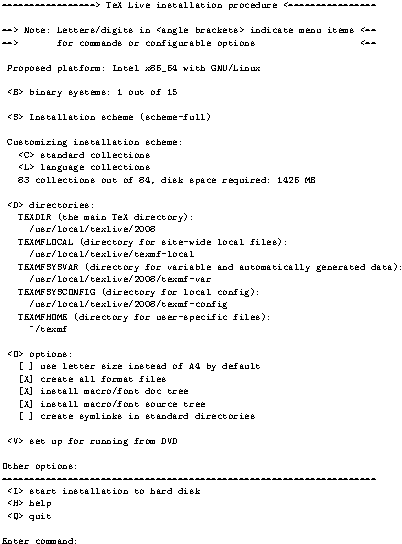
\includegraphics{install08text-crop}}
  &
 \resizebox{0.5\columnwidth}{!}{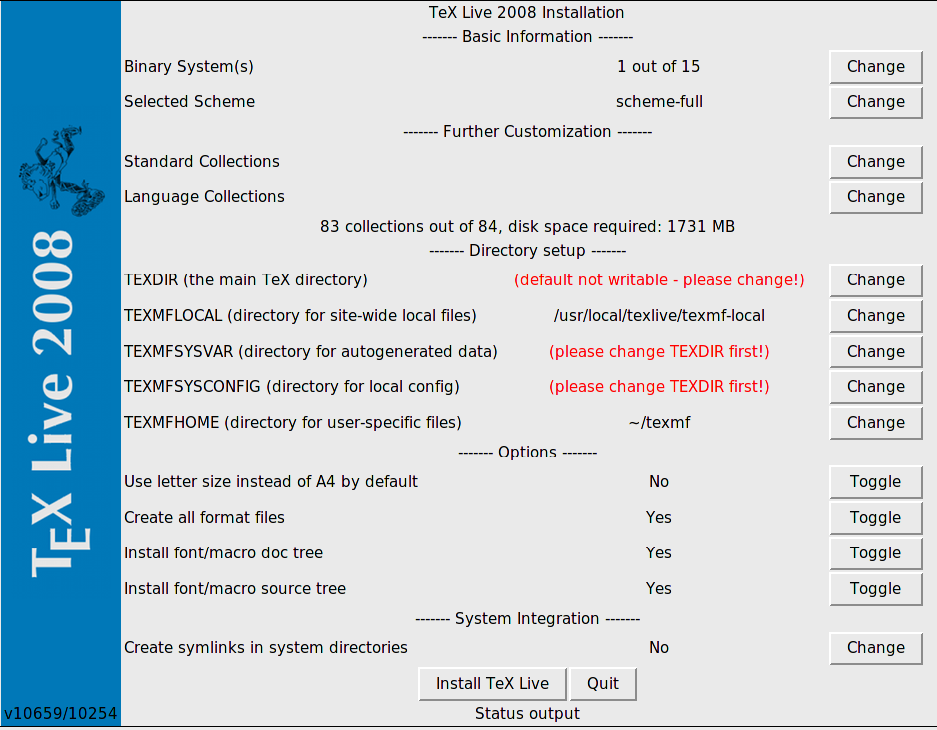
\includegraphics{gui-installer.png}}
  \end{tabular}
\end{frame}

\subsection{\tlmgr}

\begin{frame}
  \begin{center}
    \Large The new player\\[\bigskipamount]
    \tlmgr
  \end{center}
\end{frame}

\begin{frame}
  \frametitle{\TeX\ Live Manager \texttt{tlmgr}}
  \begin{itemize}
  \item installation/removal of additional packages or collections
  \item update all packages to the newest versions available
  \item backups and restore
  \item paper configuration like texconfig, but also for Windows
  \item managing the installed binary systems
  \item searching the installed and all available packages
  \item list and searching all schemes, collections, packages
  \item setting some default values like the installation location
  \item regenerate fmtutil.cnf, language.dat, and updmap.cfg from the
    information stored in the database and local additions
  \end{itemize}
\end{frame}

\begin{frame}
  \frametitle{\tlmgr\ -- Syntax}
  \begin{center}
    \texttt{tlmgr \alt<2>{\cred{[opt]...}}{[opt]...} \alt<3>{\cred{action}}{action} [opt]... [arg]...}
  \end{center}
  \only<2>{
  With first set of options:
  \begin{itemize}
  \item \url{-location} installation source, see above
  \item \url{-gui} starts the \acro{GUI}
  \item \url{-gui-lang} should be auto-detected, can be overridden
  \item standard options \url{-help}, \url{-q}, \url{-v},
    \url{-version} 
  \end{itemize}
  }
  \only<3>{
  \begin{itemize}
  \item general actions: search, show, list, uninstall, check, gui,
    version, help\bigit
  \item configuration actions: option, paper, generate\bigit
  \item package management actions: install, update, remove, backup,
    restore, arch
  \end{itemize}
  }
\end{frame}

\begin{frame}
  \frametitle{The search (and show) action}
  \begin{center}
    \texttt{tlmgr [opt]... search \cred{[opt]... what}}
  \end{center} 
  searches the \emph{locally} installed package names and descriptions
  for \texttt{\cred{what}}.

  Options:
  \begin{itemize}
  \item \texttt{-global} also searches the remote database
  \item \texttt{-file} searches for file names
  \end{itemize}
  \pause
  \begin{center}
    \texttt{tlmgr [opt]... show \cred{what}}
  \end{center} 
  shows information on the given packages
\end{frame}

\begin{frame}
  \frametitle{The install action}
  \begin{center}
    \texttt{tlmgr [opt]... install \cred{[opt]... what}}
  \end{center} 
  installs the package \texttt{what} including all dependencies

  Options:
  \begin{itemize}
  \item \texttt{-no-depends} do not install dependencies
  \item \texttt{-no-depends-at-all} do not even install architecture
    specific sub-packages
  \end{itemize}
\end{frame}

\begin{frame}
  \frametitle{The update action}
  \begin{center}
    \texttt{tlmgr [opt]... update \cred{[opt]... what}}
  \end{center} 
  installs the package \texttt{what} including all dependencies

  Options:
  \begin{itemize}
  \item \texttt{-list} list packages to be updated (or added) with
    revisions 
  \item \texttt{-all} update everything
  \item \texttt{-dry-run} don't actually do it
  \item \texttt{-backupdir dir} saves a snapshot of the current status to
    the specified directory
  \item \texttt{-no-depends}, \texttt{-no-depends-at-all} as before
  \end{itemize}
\end{frame}


\begin{frame}[plain]
  \frametitle{The \acro{GUI} of the \tlmgr}
  
  \begin{figure}[ht!]
    \centering
    \resizebox{\columnwidth}{!}{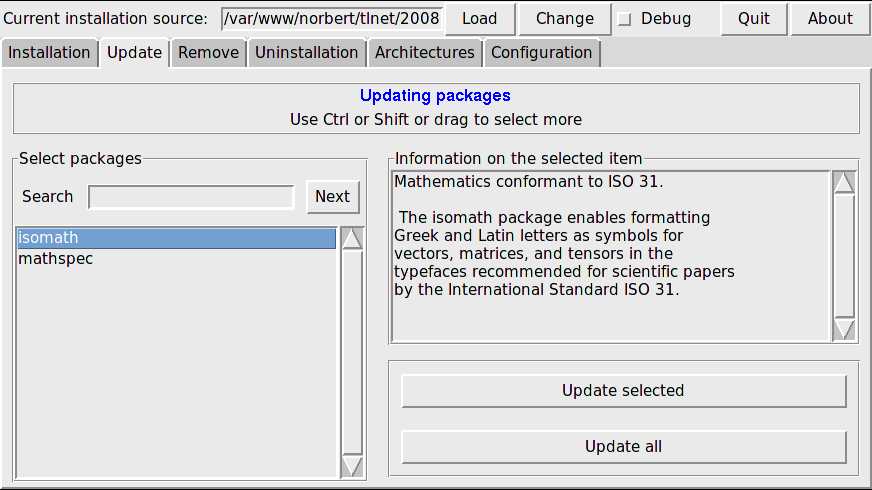
\includegraphics{tlmgrgui-update.png}}
  \end{figure}
\end{frame}

\begin{frame}
  \frametitle{Concluding remarks on \texttt{tlmgr}}
  \begin{itemize}
  \item very much work in progress, please do update your tlmgr
    immediately after a new installation
    \pause
  \item the \acro{GUI} needs a lot of work, does not exhibit all the
    functionality of the cmd line version
    \pause
  \item Perl programmers -- join us!
  \end{itemize}
  \pause
  Recovering from crashed \texttt{tlmgr} or perl modules\pause
  \begin{itemize}
  \item for Windows systems: \ctan: \texttt{update-tlmgr-latest.exe}
    \uncover<5-5>{\img{update-tlmgr-w32.png}{95pt}{-200pt}{-140pt}%
      \img{update-tlmgr-finish.png}{95pt}{-50pt}{-140pt}}
    \pause\bigit
  \item for Unix systems: \ctan: \texttt{update-tlmgr-latest.sh}
  \end{itemize}
\end{frame}


\subsection{Other news}

\begin{frame}
  \frametitle{Other (user visible) news}
  \begin{itemize}
  \item \cblue{hyph-utf8:} all engines share the same patterns\pause
  \item \cblue{lua\TeX:} embedded lua interpreter\pause
  \item \cblue{xindy} indexing program\pause
  \item \cblue{(W32) Perl and Ghostscript.}
    `hidden' copies, no interference with
    full-scale distributions\pause
  \item \cblue{(W32) \texttt{fc-cache}} helps \XeTeX{} to handle fonts more
    efficiently.\pause
  \item \cblue{(W32) PS\_View.} a new PostScript\\
    (and \acro{PDF} viewer
    that is free software%
    \uncover<6-6>{\img{psview.png}{120pt}{-40pt}{-160pt}}%
    \pause
  \item \cblue{(W32) dviout} \acro{DVI} previewer
    \uncover<7-7>{\img{dviout.png}{120pt}{-40pt}{-150pt}}
  \end{itemize}
\end{frame}


\section{Intermezzo for package writers}

\begin{frame}
  \begin{center}
    \huge Intermezzo for

    \bigskip
    Package writers
  \end{center}
\end{frame}

\subsection{Getting things into CTAN}

\begin{frame}
  \frametitle{Getting things into \tl}

  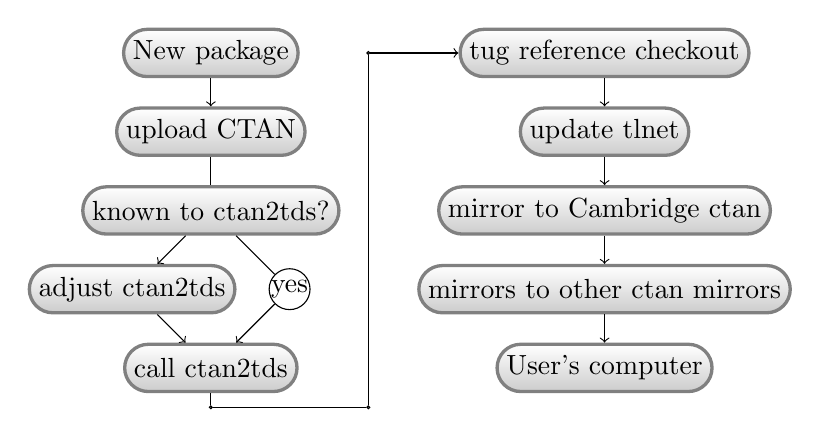
\begin{tikzpicture}[node distance=5mm,
    foo/.style={
      rectangle,minimum size=6mm,rounded corners=3mm,
      very thick,draw=black!50,
      top color=white,bottom color=black!20},
    ask/.style={
      rectangle,minimum size=6mm,rounded corners=3mm,
      very thick,draw=black!50,
      top color=white,bottom color=black!20,
      font=\itshape
    },
    point/.style={circle,draw,inner sep=0pt}]
    \node (new)  at (0,4) [foo] {New package};\pause
    \node (ctan) at (0,3) [foo] {upload CTAN};
    \path (new) edge[->] (ctan);\pause
    \node (2known) at (0,2) [ask] {known to ctan2tds?};
    \path (ctan) edge[-] (2known);\pause
    \node (temp)  at (1,1) [point] {yes};
    \path (2known) edge[-] (temp);
    \node (call) at (0,0) [foo] {call ctan2tds};
    \path (temp) edge[->] (call);\pause
    \node (adjust) at (-1,1) [foo] {adjust ctan2tds};
    \path (2known) edge[->] (adjust);
    \path (adjust) edge[->] (call);\pause

    \node (refsvn) at (5,4) [foo] {\acro{TUG} reference checkout};
    \node (p1) at (0,-0.5) [point] {};
    \node (p2) at (2,-0.5) [point] {};
    \node (p3) at (2,4) [point] {};
    \path (call) edge[-] (p1);
    \path (p1) edge[-] (p2);
    \path (p2) edge[-] (p3);
    \path (p3) edge[->] (refsvn);
    \pause

    \node (tlnet) at (5,3) [foo] {update tlnet};
    \path (refsvn) edge[->] (tlnet);
    \pause
    \node (cambridge) at (5,2) [foo] {mirror to Cambridge \acro{CTAN}};
    \path (tlnet) edge[->] (cambridge);
    \pause
    \node (mirror) at (5,1) [foo] {mirrors to other \ctan\ mirrors};
    \path (cambridge) edge[->] (mirror);
    \pause
    \node (user) at (5,0) [foo] {User's computer};
    \path (mirror) edge[->] (user);
  \end{tikzpicture}

\end{frame}

\section{Technical part}

\begin{frame}
  \begin{center}
    \huge Technical part
  \end{center}
\end{frame}

\subsection{The new infrastructure}

\begin{frame}
  \frametitle{Aims of the new infrastructure}
  \begin{itemize}
  \item Separation of static from generated content\\
    Going from a `source' to the `object' should include automatically
    data from various other sources \pause
  \item No additional files to be kept in sync\\
    any additional files tend to be outdated, all the necessary
    information should be present in \emph{one} place and be easily
    parseable. \pause
  \item Single package updates via the web\pause
  \item Better documentation\\
    since \tl\ is replacing te\TeX\ we want to give people
    incorporating \tl\ into distributions a better documented and
    easier to handle system
  \end{itemize}
\end{frame}

\begin{frame}
  \frametitle{The central \texttt{texlive.tlpdb}}
  One installation or media is now completely described by one file,
  the \TeX~Live Database:
  \begin{itemize}
  \item simple text file -- easily parseable
  \item revision number for the single packages
  \item generated from static content (the tlpsrc files)
  \item enriched with information from the \TeX~Catalogue
  \item format documented in detail (\textsc{pod} documentation in the
    respective perl module)
  \end{itemize}
\end{frame}

\begin{frame}[fragile]
  \frametitle{How does \texttt{texlive.tlpdb} look like}
  \begin{lstlisting}[title={texlive.tlpdb}]
name abbr
...

name memoir
...

\end{lstlisting}
  \begin{itemize}
  \item sequence of \texttt{key value} pairs
  \item separated by an empty line (or more)
  \item one group per package
  \item some `meta'-packages for configuration options
  \end{itemize}
\end{frame}

\begin{frame}[plain,fragile]
  \frametitle{The single package: \tlpobj\ by example I}
  \begin{lstlisting}[basicstyle=\ttfamily\tiny,title={a0poster.tlpobj},label=a0poster]
name a0poster
category Package
revision 7340
shortdesc Support for designing posters on large paper.
longdesc Provides fonts in sizes of 12pt up to 107pt and also makes sure
longdesc that in math formulas the symbols appear in the right size. Can
longdesc also create a PostScript header file for dvips which ensures
longdesc that the poster will be printed in the right size. Supported
longdesc sizes are DIN A0, DIN A1, DIN A2 and DIN A3.
docfiles size=47
 texmf-dist/doc/latex/a0poster/a0.pdf details="Package documentation (German)" language="de"
 texmf-dist/doc/latex/a0poster/a0.tex
 texmf-dist/doc/latex/a0poster/a0_eng.pdf details="Package documentation (English)" language="en"
 texmf-dist/doc/latex/a0poster/a0_eng.tex
runfiles size=4
 texmf-dist/tex/latex/a0poster/a0poster.cls
 texmf-dist/tex/latex/a0poster/a0size.sty
catalogue-version 1.22b
catalogue-date 2006-11-28 22:38:04 +0100
catalogue-ctan /macros/latex/contrib/a0poster
catalogue-license lppl
\end{lstlisting}
\end{frame}

\begin{frame}[fragile]
  \frametitle{The origin of this \texttt{a0poster.tlpobj}}
  \begin{lstlisting}[basicstyle=\ttfamily\small,title={a0poster.tlpsrc},label=a0poster.tlpsrc]
name a0poster
category Package
\end{lstlisting}
  \begin{itemize}
  \item minimal input file with static data
  \item rest is generated from actual svn repository (revision, size)
  \item enriched with information from the \TeX\ Catalogue
    (catalogue-*, specification of the documentation files)
  \item tagged documentation files (details, language), information
    again from the Catalogue
  \end{itemize}
\end{frame}

\begin{frame}[plain,fragile]
  \frametitle{The single packages: \tlpobj\ by example II}
  \begin{lstlisting}[basicstyle=\ttfamily\tiny,title={bin-bibtex8 and friends},label=bibtex8]
name bin-bibtex8
category TLCore
revision 7340
depend bin-bibtex8.ARCH
docfiles size=15
 texmf/doc/bibtex8/00readme.txt
 texmf/doc/bibtex8/HISTORY
 texmf/doc/bibtex8/csfile.txt
 texmf/doc/bibtex8/file_id.diz
runfiles size=10
 texmf-dist/bibtex/csf/base/88592pl.csf
 texmf-dist/bibtex/csf/base/cp1250pl.csf
 texmf-dist/bibtex/csf/base/cp852pl.csf
 texmf-dist/bibtex/csf/base/iso8859-7.csf

name bin-bibtex8.alpha-linux
category TLCore
revision 7340
shortdesc binary files of bin-bibtex8 for alpha-linux
binfiles arch=alpha-linux size=62
 bin/alpha-linux/bibtex8

...
name bin-bibtex8.win32
category TLCore
revision 7340
shortdesc binary files of bin-bibtex8 for win32
binfiles arch=win32 size=25
 bin/win32/bibtex8.exe
\end{lstlisting}
\end{frame}

\begin{frame}[fragile]
  \frametitle{The origin of the above \texttt{bin-bibtex8}}
  \begin{lstlisting}[basicstyle=\ttfamily\small,title={bin-bibtex8.tlpsrc},label=bin-dvipsk.tlpsrc]
name bin-bibtex8
category TLCore
runpattern d texmf-dist/bibtex/csf/base
docpattern f texmf/doc/bibtex8/*
binpattern f bin/${ARCH}/bibtex8
\end{lstlisting} % for stupid emacs: $
  \begin{itemize}
  \item various patterns for capturing files
  \item tricks to capture binaries on unix and windows
  \item separate objects for the binary files of the package
  \end{itemize}
\end{frame}

\begin{frame}[fragile]
  \frametitle{The pattern language}
  patterns are of the form
  \begin{center}
    |[PREFIX]TYPE PAT|
  \end{center}
  where |PREFIX| can be |+|, |!+|, or |!|, \pause and |TYPE PAT| can be:
  \begin{description}
  \item[f path]
    includes all files which match |path| where \emph{only} the last
    component of |path| can contain the usual glob characters * and ?
    (but no others!).\pause
  \item[d path]
    includes all the files in and below the directory specified as
    |path|.
  \end{description}
\end{frame}

\begin{frame}[fragile]
  \frametitle{The pattern language}
  patterns are of the form
  \begin{center}
    |[PREFIX]TYPE PAT|
  \end{center}
  where |PREFIX| can be |+|, |!+|, or |!|, and |TYPE PAT| can be:
  \begin{description}
  \item[t word1 ... wordN wordL]
    includes all the files in and below all directories of the form
    \begin{center}
      \path{word1/word2/.../wordN/.../any/dirs/.../wordL/}
    \end{center}\pause
  \item[r regexp]
    includes all files matching the Perl regexp \verb+/^regexp$/+
  \end{description}
\end{frame}


\begin{frame}[fragile]
  \frametitle{Example patterns}
  \begin{itemize}
  \item |runpattern f texmf/chktex/*|\\
    includes all files \emph{in} Master/texmf/chktex/\pause
  \item |binpattern f bin/${ARCH}/bibtex|\\   % for stupid emacs $
    includes the bibtex binaries into the bin-bibtex package,
    depending on the architecture\pause
  \item |runpattern d texmf/tex/lambda/base|\\
    includes all files in and under the above path\pause
  \item |runpattern t texmf-dist omega uni2char|\\
    includes all files in texmf-dist/omega/\ldots/uni2char/\pause
  \item |runpattern r .*/foobar|\\
    includes the files matching the regexp
  \end{itemize}
\end{frame}

\begin{frame}[plain,fragile]
  \frametitle{Autogenerated patterns}
  To keep \tlpsrc\ files small, if a pattern section is empty or all
  patterns are prefixed with |+|, the following patterns are
  automatically generated (actual list is specified in a special
  \tlpsrc-file): 
  \begin{itemize}
  \item runpatterns in category Package:
    \begin{center}
      |t texmf-dist topdir name|
    \end{center}
  \item docpatterns in category Package:
    \begin{center}
      |t texmf-dist doc name|
    \end{center}
  \item docpatterns in category Documentation:
    \begin{center}
      |t texmf-doc doc name|
    \end{center}
  \item srcpatterns in category Package:
    \begin{center}
      |t texmf-dist source name|
    \end{center}
  \item srcpatterns in category Documentation:
    \begin{center}
      |t texmf-doc source name|
    \end{center}
  \end{itemize}
\end{frame}

\begin{frame}[fragile]
  \frametitle{Additional tricks}

  \begin{block}{arch expansion}
  In case the string \verb+${ARCH}+ occurs in one |binpattern| it is 
  automatically expanded to the respective architecture.
  \end{block}

  \begin{block}{bat/exe/dll/texlua for win32}
    For |binpatterns| of the form |f bin/win32/foobar| files
    |foobar.bat|, |foobar.dll|, |foobar.exe|, and |foobar.texlua| are
    also matched.
  \end{block}
\end{frame}

\begin{frame}
  \frametitle{Effects of auto generation and tricks}

  total number of tlpsrc files: 1719
  
  total number of tlpsrc files with patterns: 157
  
  number of bin- and hyphen- tlpsrc files with patterns: 80
  
  number of `normal' packages with patterns: 77
\end{frame}


\begin{frame}[plain,fragile]
  \frametitle{Allowed fields for \tlpobj}
  \begin{itemize}
  \item name: identifies the package
  \item category: one of (currently) |Collection|, |Scheme|, |TLCore|,
    |Documentation|, |Package|
  \item shortdesc, longdesc: description of the package
  \item depend: |Name| (multiple entries possible)
  \item execute: activating maps, formats, hyphenation patterns
  \item runfiles, docfiles, srcfiles, binfiles\\
    every files section has a size attribute, and the
    binfiles section can occur more then once with different
    arch tags (see above)
  \item revision: maximum svn revision number of the 
    contained files, since version numbers are not
    parseable, trustworthy, or not even present
  \item catalogue-* keys: stuff taken from the catalogue\\
    for example catalogue-version, catalogue-authors, 
    catalogue-license
  \end{itemize}
\end{frame}

\begin{frame}[fragile]
  \frametitle{Perl programming \textsc{api}}
  Important for `users' or integrators
  \begin{description}
  \item[TeXLive::TLPOBJ] for \tlpobj\ files, basic
    functionality like read, write, and member access and change
    functions, etc.
  \item[TeXLive::TLPDB] access to the \tl\ database.
  \item[TeXLive::TLPostInstall] collects post installation actions
  \end{description}
\end{frame}

\begin{frame}[fragile]
  \frametitle{Perl programming \textsc{api} \acro{II}}
  Important for `us' as developer:
  \begin{description}
  \item[TeXLive::TLTREE] properties of the subversion 
    repository, in principle it is |svn status -v| 
  \item[TeXLive::TeXCatalogue] simple interface to the \TeX\
    Catalogue
  \item[TeXLive::TLPSRC] for \tlpsrc\ files, basic
    functionality like reade, write, etc
  \item[TeXLive::TLUtils] some handy functions 
  \item[TeXLive::TLMedia] abstracts an arbitrary installation media
  \end{description}
\end{frame}

\begin{frame}
  \frametitle{Other (planned/wished) \textsc{api}s}
  Are they necessary/useful? Maybe calling the Perl code \ldots?
  \begin{description}
  \item[texlua] next on the list to be done, would really help us a lot
  \item[python] minimal code present (by Jim Hefferon)
  \item[C] some code present, was a \textsc{GSoC} project, but no slot
    available (code by Jjgod Jiang)
  \item[bash] maybe, some code present (by the author)
  \item[\ldots] no idea what else \ldots
  \end{description}
\end{frame}

\begin{frame}
  \frametitle{Documentation}
  \begin{itemize}
  \item all modules contain a full documentation in pod format\bigit
  \item additional text \textsc{api} document\bigit
  \item article in Ars\TeX nica, 2007:4, 69--73, and in the
    proceedings of the Bacho\TeX~2008.
  \end{itemize}
\end{frame}


\subsection{Internals of the \tlpdb, config options}

\begin{frame}
  \frametitle{Some special packages}
  Some packages do not relate to actual files but are used to save
  options and configurations into the database by putting them into a
  depend line: \texttt{00texlive.config},
  \texttt{00texlive-installation.config},
  \texttt{00texlive.core}.

  Values are stored in these packages as dependencies.

  All packages starting with \texttt{00texlive} are considered virtual
  packages in the sense that no containers are generated and these
  packages are never split into .src and .doc sub-packages in the
  tlpdb. 
\end{frame}

\begin{frame}
  \frametitle{\texttt{00texlive.config}}
  This package contains configuration options for the \tl\ archive:
  \begin{itemize}
  \item \texttt{container\_split\_\{doc,src\}\_files}\\
    documentation and source files are split into separate containers
    (.tar.lzma) during container build time. Note that this has
    \emph{no} effect on the appearance within the texlive.tlpdb. It is
    only on container level.
  \item \texttt{container\_format/XXXXX}\\
    specifies the format, currently allowed is only \texttt{lzma}, which
    generates .tar.lzma files. zip can be supported. 
  \item \texttt{release/NNNN}\\
    specifies the release number as used in the installer
  \end{itemize}
\end{frame}

\begin{frame}
  \frametitle{\texttt{00texlive-installation.config}}
  This package serves two purposes:
  \begin{itemize}
  \item at installation time the present values are taken as default for
    the installer
  \item on an installed system it serves as a configuration file.
    We have to remember these settings for additional package
    installation, removal, etc.
  \end{itemize}
  The value of \texttt{\_\_MASTER\_\_} for the location field tells the
  installer to use the present directory itself.  For example,
  the \acro{DVD} can be mounted anywhere and we want the installer to work.
\end{frame}

\begin{frame}[fragile]
  \frametitle{Example \texttt{00texlive-installation.config}}
  \begin{lstlisting}[basicstyle=\ttfamily\small]
name 00texlive-installation.config
category TLCore
depend platform:x86_64-linux
depend location:/var/www/norbert/tlnet/2008
depend opt_paper:a4
depend opt_create_formats:0
depend opt_create_symlinks:0
depend opt_sys_bin:/usr/local/bin
depend opt_sys_info:/usr/local/info
depend opt_sys_man:/usr/local/man
depend opt_install_docfiles:1
depend opt_install_srcfiles:0
depend available_architectures:x86_64-linux win32
\end{lstlisting}
\end{frame}


\begin{frame}
  \frametitle{\texttt{00texlive.core}}
  actually contains files, but those are
  never installed and this package is only here to collect files
  which are not contained in any package, thus making the coverage
  check squeak
\end{frame}

% \begin{frame}
%   \frametitle{Organization ??????????????}
%   \begin{itemize}
%   \item \textsc{svn} repository where many people have write permissions
%   \item loads of supporting scripts doing a variety of jobs:
%     \begin{itemize}
%     \item preparing the installation for mastering
%     \item installation from various media
%     \item installation of packages from \textsc{ctan} into the
%       \textsc{svn} repository
%     \item performing various checks on the whole archive (coverage,
%       double inclusion, etc.)
%     \end{itemize}
%   \end{itemize}
% \end{frame}

\section{Closing}


\begin{frame}
  \frametitle{Resources}
  \begin{itemize}
    \item \url{tex-live@tug.org} -- main contact point
  \item \path{www.tug.org/texlive} -- the main entry point, with
  links to developers' resources, documentation
\item \path{www.tug.org/svn/texlive/trunk/} -- web view onto the
  subversion repository;
\item \path{svn://tug.org/texlive/trunk} -- svn repository, anonymous
  access
\item \path{www.tug.org/texlive/pkgupdate.html} -- an
  explanation how updates from \ctan\ to \tl\ are done.
  \end{itemize}
\end{frame}

\begin{frame}
  \begin{center}
    {\Large Thanks}

    \bigskip
    Karl Berry\\
    {\small for great enthusiasm and  perpetual
      support (and critical voices)}
    
    \pause
    \bigskip
    \acro{TUG}\\% and \acro{DANTE}\\
    {\small for financial support when my laptop broke}
    
    \pause
    \bigskip
    Your Attention
  \end{center}
\end{frame}


\end{document}
